% -*- LaTeX -*-
% -*- coding: utf-8 -*-
%
% ~~~~~~~~~~~~~~~~~~~~~~~~~~~~~~~~~~~~~~~~~~~~~~~~~~~~~~~~~~~~~~~~~~~~~~~~~~~~~~
%
%                             michael a.g. aïvázis
%                      california institute of technology
%                      (c) 1998-2010  all rights reserved
%
% ~~~~~~~~~~~~~~~~~~~~~~~~~~~~~~~~~~~~~~~~~~~~~~~~~~~~~~~~~~~~~~~~~~~~~~~~~~~~~~
%

\lecture{Cost modeling and performance tradeoffs}{20100113}

% --------------------------------------
% generic parallel architecture
\begin{frame}[fragile]
%
  \frametitle{Time, parallelism and computational work}
%
  \begin{itemize}
  \item recall our embarrassingly parallel reduction: 
    \begin{itemize}
    \item given a function $f$ and a sequence of numbers $S$ of length $N$, evaluate
    \[
    s = \sum_{i=0}^{N-1}f(S_{i})
    \]
    \end{itemize}
%
  \item initial parallelism profile for a simple mapping, assuming that
    \begin{itemize}
    \item the computation of $f(S)$ is the parallel task
    \item the summation is sequential
    \end{itemize}
%
    \begin{minipage}{.45\linewidth}
      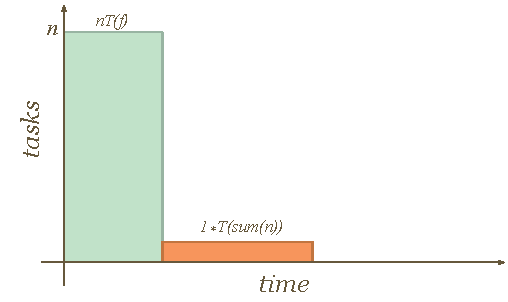
\includegraphics[scale=0.6]{figures/reduction-parallel-work.pdf}
    \end{minipage}
    $\longrightarrow$
    \begin{minipage}{.45\linewidth}
      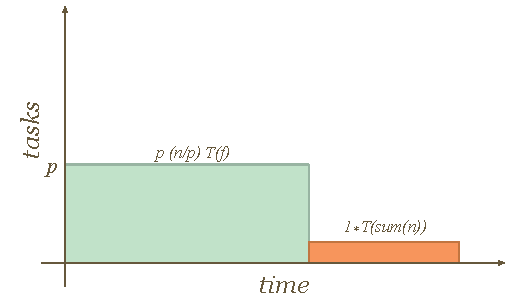
\includegraphics[scale=0.6]{figures/reduction-partitioned-work.pdf}
    \end{minipage}
%
  \item shaded area is $w$, the {\em computational work}
%
  \end{itemize}
%
\end{frame}

% --------------------------------------
% speedup and efficiency
\begin{frame}[fragile]
%
  \frametitle{Metrics: speedup and efficiency}
%
  \begin{itemize}
%
    \item let
      \begin{itemize}
        \item $T_{1}$ be the sequential execution time on one processor
        \item $T_{p}$ be the parallel execution time on $p$ processors
      \end{itemize}
%
    \item define
      \begin{itemize}
        \item {\em speedup}: \[\sigma \defeq T_{1}/T_{p}\]
        \item {\em efficiency}: \[\eta \defeq T_{1}/(p T_{p})\]
        \item related through $\eta = \sigma/p$ and $\sigma = \eta p$
      \end{itemize}
%
    \item pseudo-theorems: $\sigma \leq p$ and $\eta \leq 1$
      \begin{itemize}
        \item but {\em speedup anomalies} can occur if resources increase with $p$ causing an
          increase in the effective computation rate
        \item example: for large enough $p$, your problem may fit entirely in the L2 cache
        \item {\em sweet spots} like that abound; the craftsman knows how to
          \begin{itemize}
            \item implement the solution in a portable manner
            \item expose enough controls to be able to tune the implementation to a given
              architecture
          \end{itemize}
      \end{itemize}
%
  \end{itemize}
%
\end{frame}

% --------------------------------------
% amdahl's law
%
\begin{frame}[fragile]
%
  \frametitle{The bad news: Amdahl's law}
%
  \begin{itemize}
%
  \item consider a solution that consists of two parts
    \begin{itemize}
    \item a serial fraction $s$ with $0 \leq s \leq 1$
    \item a $p$-fold parallel fraction $1-s$
    \end{itemize}
%
  \item for a fixed problem size, Amdahl's law relates $T_{p}$, $\sigma$ and $\eta$ to $T_{1}$
    and $s$

    \begin{eqnarray*}
      T_{p}  & = & s T_{1} + (1-s) T_{1} / p \\
      \sigma & = & \frac{p}{sp + (1-s)} \\
      \eta & = & \frac{1}{sp + (1-s)}
    \end{eqnarray*}

%
\item with corollaries $\sigma_{\infty} = \frac{1}{s}$ and $\eta_{\infty} = 0$

    \begin{minipage}{.45\linewidth}
      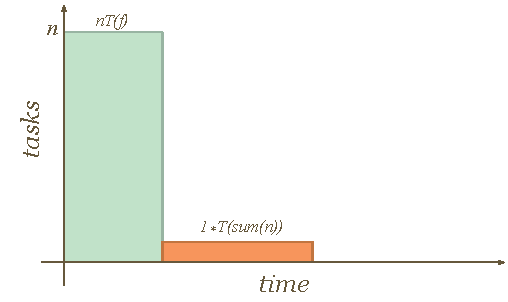
\includegraphics[height=1in]{figures/reduction-parallel-work.pdf}
    \end{minipage}
    \hfill
    \begin{minipage}{.45\linewidth}
      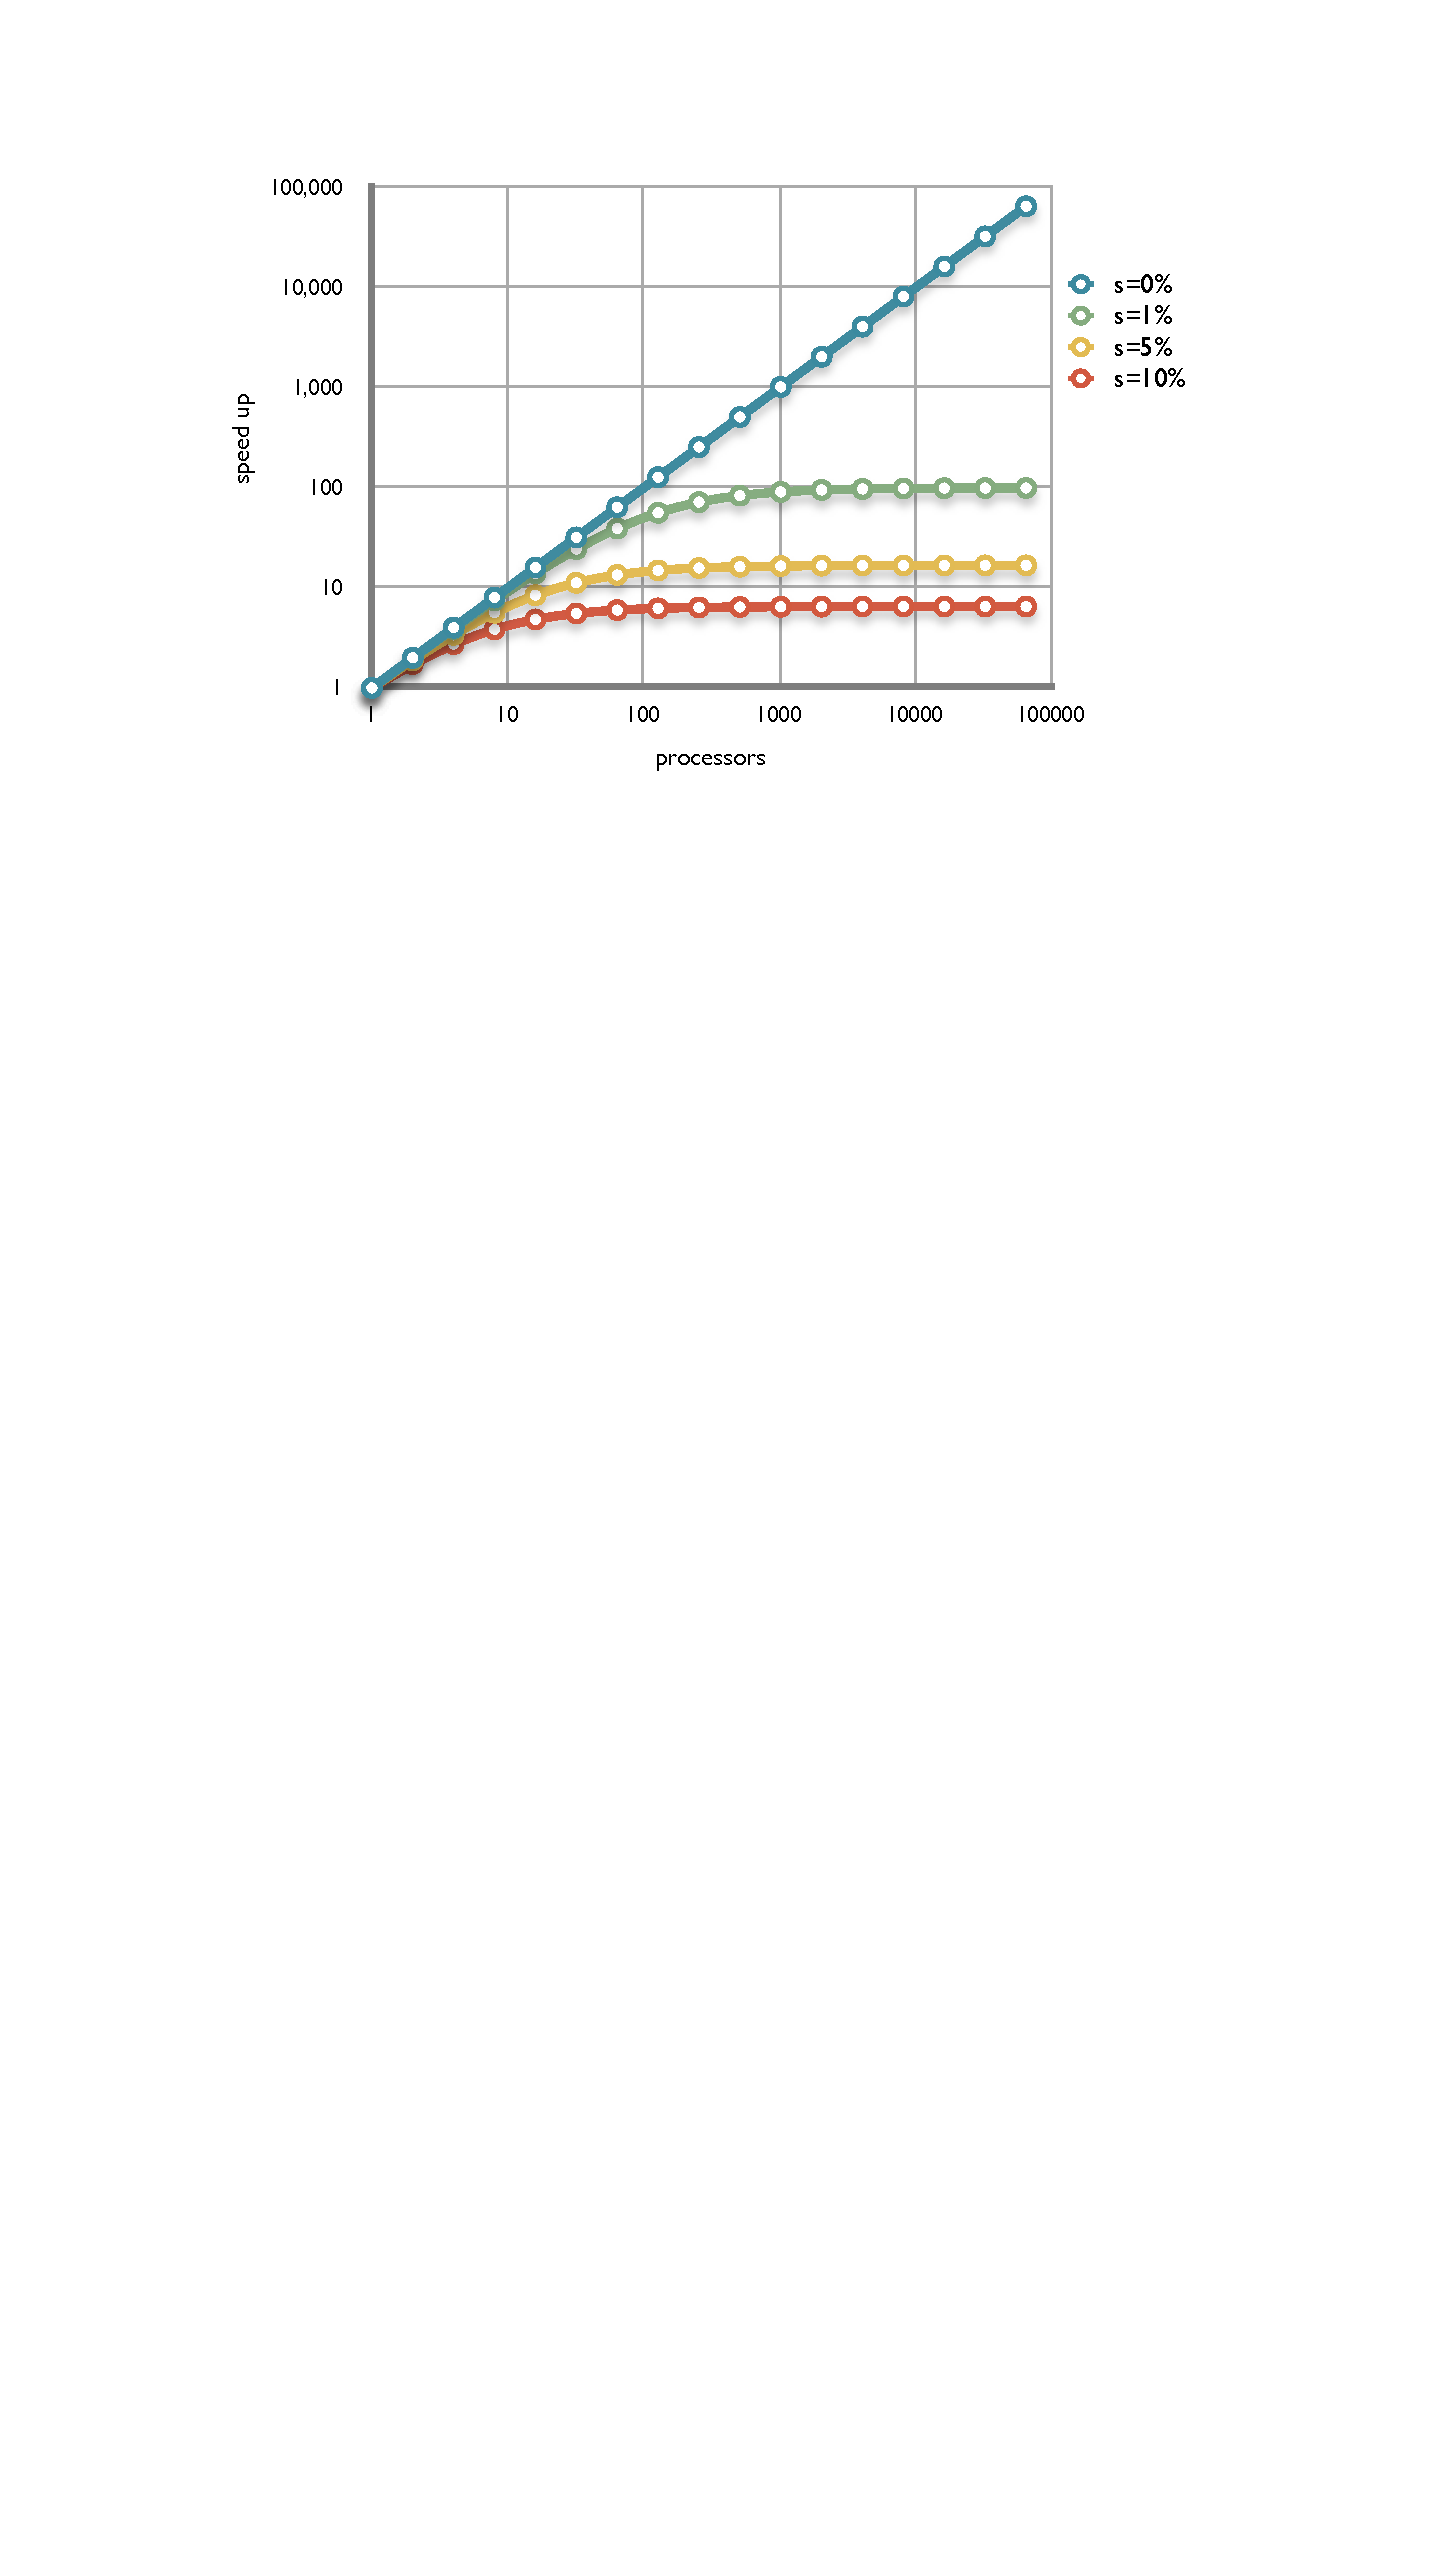
\includegraphics[height=.9in]{figures/amdahl.pdf}
    \end{minipage}

%
  \end{itemize}
%
\end{frame}

% --------------------------------------
% scaling and isoefficiency
\begin{frame}[fragile]
%
  \frametitle{Beating Amdahl's law}
%
  \begin{itemize}
  \item Amdahl's law holds if either
    \begin{itemize}
      \item the problem size is fixed
      \item the serial fraction $s$ is not a function of $p$
    \end{itemize}
%
  \item {\em weak scaling}: let the problem size grow with $p$
    \begin{itemize}
    \item larger computers are used to solve larger problems
    \item the effective serial fraction {\em decreases} with problem size
    \item the right scaling metric would be constant, or properly bounded, as $p \rightarrow
      \infty$
    \end{itemize}
%
  \item {\em isoefficiency}
    \begin{itemize}
      \item how rapidly must problem size grow so that $\eta$ is constant as $p$ increases?
      \item since $\eta = T_{1}/(pT_{p})$, constant efficiency implies
        \[
        T_{1} = c (p T_{p})
        \]
        for some constant $c$
      \item $T_{1}$ measures the sequential work, so the above relation determines your
        implementation's {\em isoefficiency function}
    \end{itemize}
%
  \end{itemize}
%
\end{frame}



% --------------------------------------
% algorithmic trade-offs
\begin{frame}[fragile]
%
  \frametitle{Algorithmic improvements}
%
  \begin{itemize}
%
  \item getting smarter is the best way to improve $\sigma$ and $\eta$
    \begin{itemize}
      \item reduce the sequential fraction $s$
      \item what are the effects on communication and locality?
    \end{itemize}
%
  \item parallelize the partial sums
    \begin{figure}
      \centering
      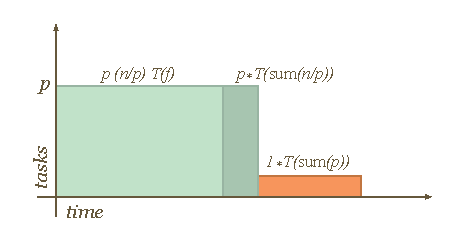
\includegraphics[scale=0.70]{figures/reduction-partial-sum.pdf}
    \end{figure}
%
  \item parallelize the final sum using a {\em reduction tree}
    \begin{figure}
      \centering
      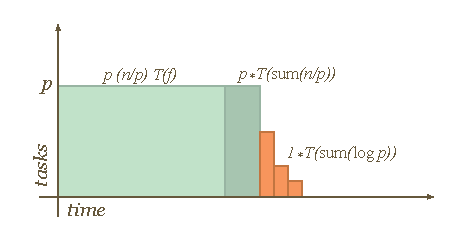
\includegraphics[scale=0.70]{figures/reduction-tree-sum.pdf}
    \end{figure}
%
  \end{itemize}
%
\end{frame}

% --------------------------------------
% load balance
\begin{frame}[fragile]
%
  \frametitle{Load balance}
%
  \begin{itemize}
%
  \item non-optimal task distributions show up as {\em load imbalance}
    \begin{figure}
      \centering
      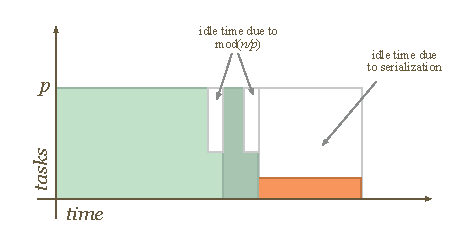
\includegraphics[scale=1.0]{figures/reduction-load-imbalance.pdf}
    \end{figure}
%
  \item excessive coarsening tends to increase load imbalance
  \item so can inappropriate mapping
  \item synchronization also causes load imbalance (see later slide)
  \item new upper bound for the speedup
    \[
    \sigma \leq \frac{w_{1}}{{\rm max\ }_{p}(w_{p} + {\rm idle})}
    \]
      
  \end{itemize}
%
\end{frame}

% --------------------------------------
% overhead
\begin{frame}[fragile]
%
  \frametitle{Parallelization overhead}
%
  \begin{itemize}
%
  \item there is always some extra work that is not present in the sequential implementation
    \begin{figure}
      \centering
      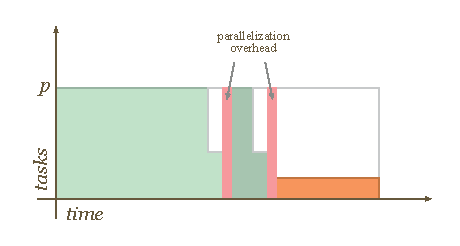
\includegraphics[scale=1.0]{figures/reduction-overhead.pdf}
    \end{figure}
%
  \item orchestration, management, bookkeeping
    \[
    \sigma \leq \frac{w_{1}}{{\rm max\ }_{p}(w_{p} + {\rm idle} + {\rm overhead})}
    \]
      
%
  \end{itemize}
%
\end{frame}

% --------------------------------------
% communication and synchronization costs
\begin{frame}[fragile]
%
  \frametitle{Communication and synchronization costs}
%
  \begin{itemize}
%
  \item communication is required for data movement and synchronization
    \begin{figure}
      \centering
      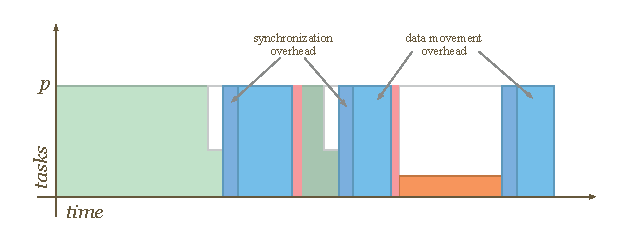
\includegraphics[scale=0.75]{figures/reduction-comsync.pdf}
    \end{figure}
%
  \item the cost is modeled by
    \[
    T_{c} = \lambda + \beta L
    \]
    where the {\em latency} $\lambda$ measures the communication startup cost, $\beta$ is the
    bandwidth of the interconnect and $L$ is the message length in {\em words} 
%
  \item the speedup is now bounded by
    \[
    \sigma \leq \frac{w_{1}}{{\rm max\ }_{p}(w_{p} + {\rm idle} + {\rm overhead} + {\rm comm})}
    \]
%      
  \end{itemize}
%
\end{frame}

% --------------------------------------
% reducing communication costs
\begin{frame}[fragile]
%
  \frametitle{Reducing communication costs}
%
  \begin{itemize}
%
  \item multiple strategies
%
  \item co\"ordinating placement of work and the associated data to minimize inter-process
    dependencies
    \begin{figure}
      \centering
      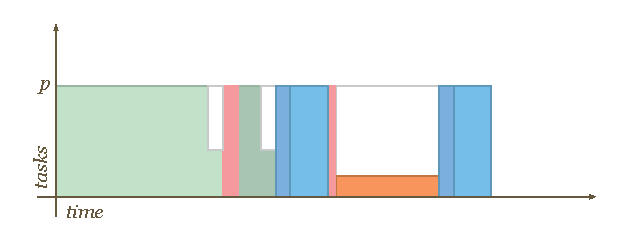
\includegraphics[scale=0.5]{figures/reduction-comsync-replication.pdf}
    \end{figure}
%
  \item trading memory for efficiency by replicating data
%
  \item trading cpu for efficiency by doing redundant work
    \begin{figure}
      \centering
      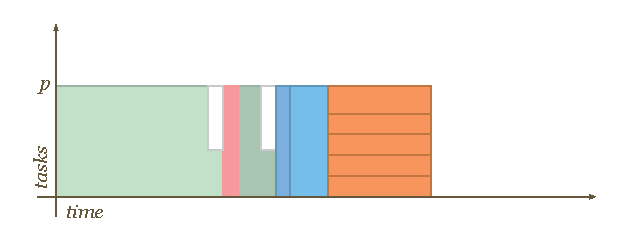
\includegraphics[scale=0.5]{figures/reduction-comsync-redundancy.pdf}
    \end{figure}
%
  \item improving communication efficiency by tuning the cost factors
    \begin{itemize}
    \item communication frequency, message size, contention, architecture specific
      optimizations
    \end{itemize}
%
  \end{itemize}
%
\end{frame}

% --------------------------------------
% tension
\begin{frame}[fragile]
%
  \frametitle{Optimizing speedup and efficiency}
  \begin{itemize}
%
    \item the goal is to minimize the denominator
      \[
      \sigma \leq \frac{w_{1}}{{\rm max\ }_{p}(w_{p} + {\rm idle} + {\rm overhead} + {\rm comm})}
      \]
      \begin{itemize}
        \item but its parts are in tension: minimizing one happens at the expense of another
      \end{itemize}
%
  \item fine grain decomposition and intelligent mapping tend to minimize load imbalance at the
    cost of increased communication
    \begin{itemize}
    \item coarser grains imply larger message size and fewer synchronization events
    \item for many problems communication costs decrease as surface to volume
    \end{itemize}
%
  \item na\"ive static partitioning reduces redundant work but cause load imbalance
%
  \end{itemize}
%
\end{frame}

% --------------------------------------
% the good news
\begin{frame}[fragile]
%
  \frametitle{The good news}
%
  \begin{itemize}
%
  \item the basic work unit of a parallel algorithm may be more efficient (and better
    performing) than the sequential equivalent
    \begin{itemize}
    \item only a small fraction of typical problems fits in L2 cache
    \item single node performance {\em requires} partitioning
    \item just like the parallel implementation
    \item don't be surprised by the poor quality of your sequential version after you see
      your parallel implementation
    \end{itemize}
%
  \item communication can be interleaved with computation
    \begin{itemize}
    \item better algorithms on today's complicated memory hierarchies
    \end{itemize}
%
    \item parallel algorithms may lead to better sequential ones
      \begin{itemize}
        \item e.g.~parallel search may explore configuration space more effectively
      \end{itemize}
%
  \end{itemize}
%
\end{frame}

% end of file 
